\documentclass[parskip=half, titlepage=firstiscover, captions=tableheading, bibliography=totoc]{scrartcl}
%optionen immer variieren tabelheading bei tabellen
%ohne parskip nur einrücken
%draft macht hüllen von bilder selbst wenn sie nicht existieren um einfach zeit bei compilieren zu sparen
%\usepackage{scrhack} % nach \documentclass
\usepackage{float}
\floatplacement{figure}{htbp}
\floatplacement{table}{htbp}
\usepackage[aux]{rerunfilecheck}
\usepackage{polyglossia}
\usepackage{biblatex}
\addbibresource{Tag3.bib}%name der bib-Datei hier einfügen !
\setmainlanguage{german}
\usepackage{longtable}
\usepackage{amsmath}
\usepackage{amssymb}
\usepackage{mathtools}
\usepackage{fontspec}
\usepackage[
math-style=ISO,
bold-style=ISO,
sans-style=italic,
nabla=upright,
partial=upright,
]{unicode-math}

\setmathfont{Latin Modern Math}
\usepackage{graphicx}
\usepackage{grffile}
\usepackage[font = scriptsize, labelfont = bf,margin={10pt,10pt}]{subcaption}
\usepackage[font = scriptsize, labelfont = bf,margin={10pt,10pt}]{caption}
%anstatt margin geht auch width = 10cm
\usepackage{mleftright}
%schöneres mit  \mleft (\mright)

\setlength{\delimitershortfall}{-1sp}
%bei vielen Klammern werden sie nun größer
\usepackage[locale=DE,separate-uncertainty=true,per-mode=symbol-or-fraction]{siunitx}
\usepackage{booktabs}
\usepackage{xfrac}
\usepackage{pdflscape}
%-> dazu wäre begin{landscape} etc nötig

%nur ein beispiel zu dieser änderung wenn man will
%gleiche sachen werden bei mathe oder text anders benutzt
%\let\vaccent=\v % alten Befehl kopieren
%\RenewDocumentCommand \v {} % Befehl überschreiben
%{
%\TextOrMath{
%\vaccent % Textmodus
%}{
%\symbf % Mathemodus
%}
%}

%\NewDocumentCommand \OverfullCenter {+m} {
%\noindent\makebox[\linewidth]{#1} }
%bei zu breiten pics zentrierte ausrichtung
%zu befehl wäre dann: \OverfullCenter{\includegraphics[width=\textwidth+15pt]{figures/
%Panorama.jpg}}

\AtBeginDocument{ % wird bei \begin{document} ausgeführt
\let\symIm=\Im % werden sonst wieder von unicode-math überschrieben
\RenewDocumentCommand \Re {}
{
\operatorname{Re}
}
\let\symIm=\Im
\RenewDocumentCommand \Im {}
{
\operatorname{Im}
}
}


\usepackage{fontspec}%nach amssymb
\usepackage[unicode]{hyperref}
\usepackage[shortcuts]{extdash} % nach hyperref, bookmark am Ende!
\usepackage{bookmark}

\begin{document}
\section{Auswertung}

Alle Diagramme und die lineare Ausgleichsrechnung der Auswertungen werden mit "Gnuplot" angefertigt.
Die erste Messreihe, die aufgenommen wird, ist die Geschwindigkeit der einzelnen
Stufen des Wagens. Die Strecke zwischen den Lichtschranken zur Zeitmessung
ist mit $32,7 cm$ ermittelt. Mit den gemittelten Durchlaufzeiten(Tabelle 1) werden die
Geschwindigkeiten der Einraststufen des Apparats durch $ v = s/t $ errechnet und ebenfalls in die Tabelle einetragen.
Die mittleren Fehler der Zeiten belaufen sich auf $\pm{0,002}$ und die der Geschwindigkeit, die sich durch das restliche Experiment zieht auf $\pm{0,001}$
\\
\begin{table}
\centering
 \caption{Zeiten und Geschwindigkeiten des Wagens}
\label{tab:geschwin}
\begin{tabular}{ c c c }
\toprule
"Stufe" & $\overline{t}/s$ & $v/\si{\meter\per\sec}$ \\
\midrule
6 & 6,5382 & 0.0500 \\
12 & 3,2664 & 0.1001 \\
18 & 2,1814 & 0.1499\\
24 & 1,6313 & 0.2004\\
30 & 1,3072 & 0.2502\\
36 & 1,0902 & 0.3000\\
42 & 0,9338 & 0.3502\\
48 & 0,8177 & 0.4000\\
54 & 0.7272 & 0.4500\\
60 & 0.6557 & 0.4990\\
\bottomrule
\end{tabular}
\end{table}
\\
Mit Hilfe der gemessenen Ruhefreuquenz $\nu_0 = \SI{20742}{\hertz}$ werden die
Eingangsfrequenz mit () auf $\nu_E = \SI{20770,979(100)}{\hertz}$ sowie die Ausgangsfrequenz mit ()
auf $\nu_A = \SI{20771,012(100)}{\hertz}$ errechnet.
Desweiteren wird die Grundfrequenz mit der, durch den Präzisonsschlitten und dem
Nutzen von Lissajoufiguren ermittelten und gemittelten Wellenlängen
$\overline{\lambda} = 0,01712 \pm{0,0002} m $ durch $ c = \nu_0\lambda$ zur Schallgeschwindigkeit von $\SI{355,103}{\meter\per\sec}$
berechnet.
\\
Als nächstes werden die Frequenzen bei verschiedenen Stufen der Fahrkonstruktion gemessen.
Mit den aus Tabelle 2 und 3 entnommenen Mittlungen dieser werden die Frequenzdifferenzen $\Delta\nu$
gegen die schon zuvor ausgerechten Geschwindigkeiten (Tabelle 1) in das Diagramm 1 aufgetragen.
Hierbei ist anzumerken, dass Frequenzen bei Verringerung des Abstandes Mikrofon und Lautsprecher
mit postiven Geschwindigkeiten und die Rückfahrt mit negativen zusammen geführt werden.
\\
\begin{table}
\centering
 \caption{Frequenzen und ihre Differenzen bei Verringerung des Abstandes (positiv)}
\label{tab:pos}
\begin{tabular}{ c c c }
\toprule
Stufe & $\overline{\nu}/Hz$ & $\Delta\nu/Hz$ \\
\midrule
6 & 20745,0 & 3,0 \\
12 & 20748,0 & 6,0 \\
18 & 20751,2 & 9,2\\
24 & 20754,0 & 12,0\\
30 & 20757,0 & 15,0\\
36 & 20760,6 & 18,6\\
42 & 20763,4 & 21,4\\
48 & 20766,2 & 24,2\\
54 & 20769,2 & 27,2\\
60 & 20772,2 & 30,2\\
\bottomrule
\end{tabular}
\end{table}
\begin{table}
\centering
 \caption{Frequenzen und ihre Differenzen bei Erhöhung des Abstandes (negativ)}
\label{tab:neg}
\begin{tabular}{ c c c }
\toprule
Stufe & $\overline{\nu}/Hz$ & $\Delta\nu/Hz$ \\
\midrule
-6 & 20739,0 & 3,0 \\
-12 & 20736,0 & 6,0 \\
-18 & 20733,0 & 9,0\\
-24 & 20730,0 & 12,0\\
-30 & 20727,0 & 15,0\\
-36 & 20724,0 & 18,0\\
-42 & 20720,8 & 21,2\\
-48 & 20718,0 & 24,0\\
-54 & 20715,0 & 27,0\\
-60 & 20712,0 & 30,0\\
\bottomrule
\end{tabular}
\end{table}
\newpage
\begin{figure}
  \centering
  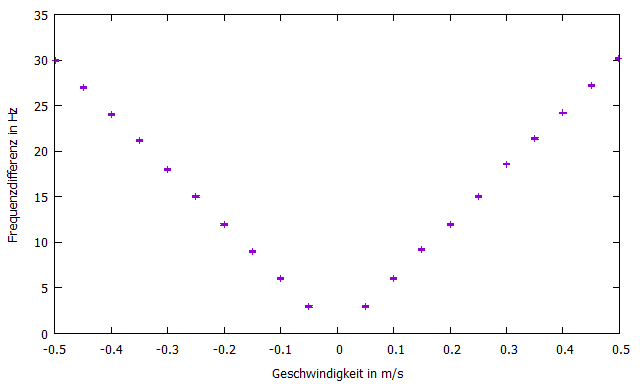
\includegraphics[width=\textwidth]{diagramD.jpg}
  \caption{Die Auftragung Geschwindigkeit $v$ zu Frequenzdifferenz $\Delta\nu$ mit dem Fehler $0,1 Hz$}
  \label{fig:DiaD}
\end{figure}
Aus diesem Diagramm lässt sich mit Hilfe der linearen Ausgleichsrechnung die Proportionnaltitätsfaktoren(bzw. Steigung)
auf $-0,845 Hz s/m$ beim negativen Anteil und $+0,845 Hz s/m$ beim postiven Anteil der Auftragung ermitteln.
\newpage
Als letzter Teil des Experiments wird die Schwebung betrachtet.
Nach Umbauen des Schaltnetztes, sowie Befestigen einer Refelectorplatte auf den Wagen, kann nun direkt die Frequenzdifferenz gemssen werden.
Mit diesen Werten (Tabelle 4) und den Geschwindigkeiten des Wagens (Tabelle 1) wird wieder $v$ zu $\Delta\nu$ ein Diagram (2) aufgetragen.
Hierbei muss beachtet werden, dass es sich um entweder die doppelte Strecke und damit halbe Geschwindigkeit oder die gemessenen Differenzen noch halbiert werden müssen.
\begin{table}
\centering
 \caption{Frequenzdifferenzen beim Vergrößern des Abstandes des Reflektors zur Quelle}
\label{tab:ref}
\begin{tabular}{ c c }
\toprule
Stufe & $\Delta\nu/Hz$ \\
\midrule
-6 & 6,0\\
-12 & 12,0 \\
-18 & 19,2\\
-24 & 25,0\\
-30 & 30,8\\
-36 & 36,0\\
-42 & 42,0\\
-48 & 47,8\\
-54 & 53,6\\
-60 & 60,0\\
\bottomrule
\end{tabular}
\end{table}
\newpage
\begin{figure}
  \centering
  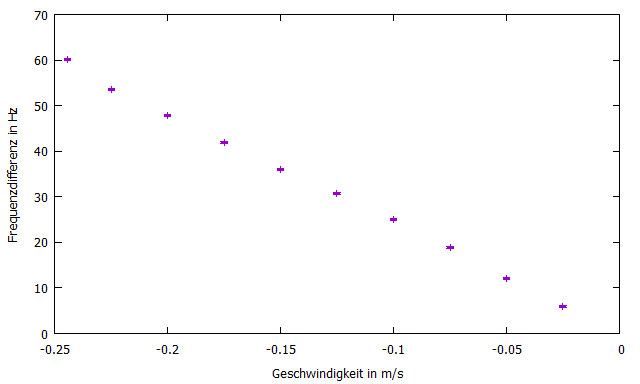
\includegraphics[width=\textwidth]{DiagramE.jpg}
  \caption{Die Auftragung Geschwindigkeit $v$ zu Frequenzdifferenz $\Delta\nu$ mit dem Fehler $\pm 0,2 Hz$\\ bei Nutzung des Reflektors.}
  \label{fig:DiaE}
\end{figure}
Auch hier wird mit Hilfe der Ausgleichsrechnung die Steigung und damit der Proportionalitätsfaktor errechnet auf einen Wert von $-0,888 HZ s/m $
\newpage
\section{Diskussion}
Die erste Untersuchung die zu machen ist, ist die um die Eingangs und Ausgangsfrequenz.
Diese unterscheiden sich bei der Rechnung, um etwas mehr als $ 1 Hz$, was beim theoretischen Wert zwar einen Unterschied macht, dieser doch so gerring ist, dass es sich kaum und dann nur im Fehlertoleranzbereich auf das Experiment auswirkt.
Die Fehler hierbei sind deutlich durch das ungenaue Messen der Strecke und damit Fehler in der Geschindigkeit zu begründen.
Das ungenaue Ablesen und die damit verbundene Unsicherheit beim Präzisionsschlitten wirkt sich auch auf die Errechnung der Schallgeschwindigket aus, die sich vom Literaturwert von $\SI{344}{\m\per\sec}$[2] um ungefähr $11 m/s$ unterscheidet.
Weitere Messungen der Frequenzen bei verschiedenen Geschwindigkeiten, sind durch die Möglichkeit der genauen Zeitmessung durch die Lichtschranken deutlich präziser.
Zusätzlich ber der letzten Messreihe sind durch die Überlagerung der Wellen, der Schwebung, die Ungenauigkeit zu erklären.

Literatur
[2] www.lefiphysik.de/themenbereiche/schallgeschwindigkeit
\end{document}
